

\chapter{Sistema de controlo e monitorização}


A plantação da salicórnia carece de um controlo relativamente fino da salinidade do terreno onde ela cresce. A salinidade do terreno depende, por sua vez, das chuvas, da salinidade da água dos canais da ria, etc. Nas “quintas” de salicórnia da Ria, a produção faz-se numa espécie de leiras limitadas por pequenos canais de irrigação. Esses canais podem ser cheios de água salgada proveniente dos esteiros que rodeiam a “quinta”. Essa operação implica a abertura de válvulas de admissão dessa água, medida do nível da maré nos canais, monitorização da qualidade e salinidade da água exterior.
Por sua vez, a cultura pode ser ameaçada por excesso de água doce de chuvas ou ser objeto de vandalismo.





\begin{figure}[!htb]
	\centering
	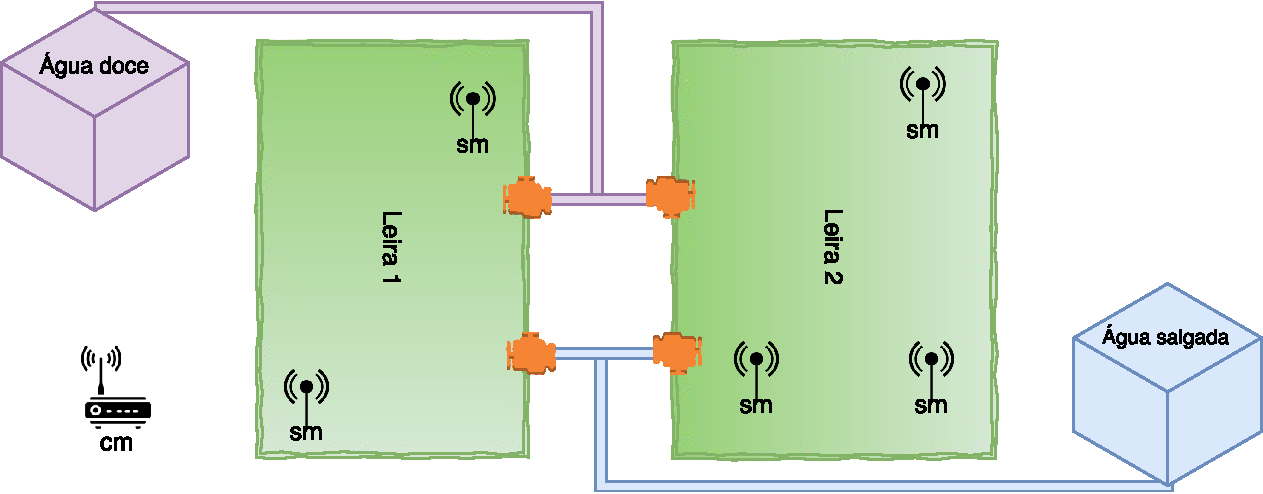
\includegraphics[scale=0.55]{esquemas/leiras-comm-geral.pdf}
	\caption{Pirâmide do conhecimento: modelo DIKW}
	\label{dikw}
\end{figure}


\section{Design funcional}











\subsection{Requisitos funcionais}


Os requisitos funcionais especificam os critérios que devem ser usados ​​para avaliar comportamentos ou funções especificas do sistema. Estes são os requisitos funcionais do sistema proposto nesta dissertação. 


A interface do sistema deve permitir que o usuário faça login no sistema
Admin ou um usuário.


A interface do sistema deve permitir que o usuário saia do sistema.



O sistema deve permitir o armazenamento de informações do cliente.


O sistema deve permitir a atualização das informações do cliente.


\subsection{Requisitos não funcionais}







\section{Design técnico}



\subsection{Arquitetura do sistema}



\subsubsection{Camada de apresentação}


\subsubsection{Camada de negócio}



\subsubsection{Camada de dados}




\section{Diagrama de componentes}




\section{Sistema de interação}


\section{Descrição}


Modulos da daniela : Cc1110



\section{Arquitetura geral}

\begin{figure}[!htb]
	\centering
	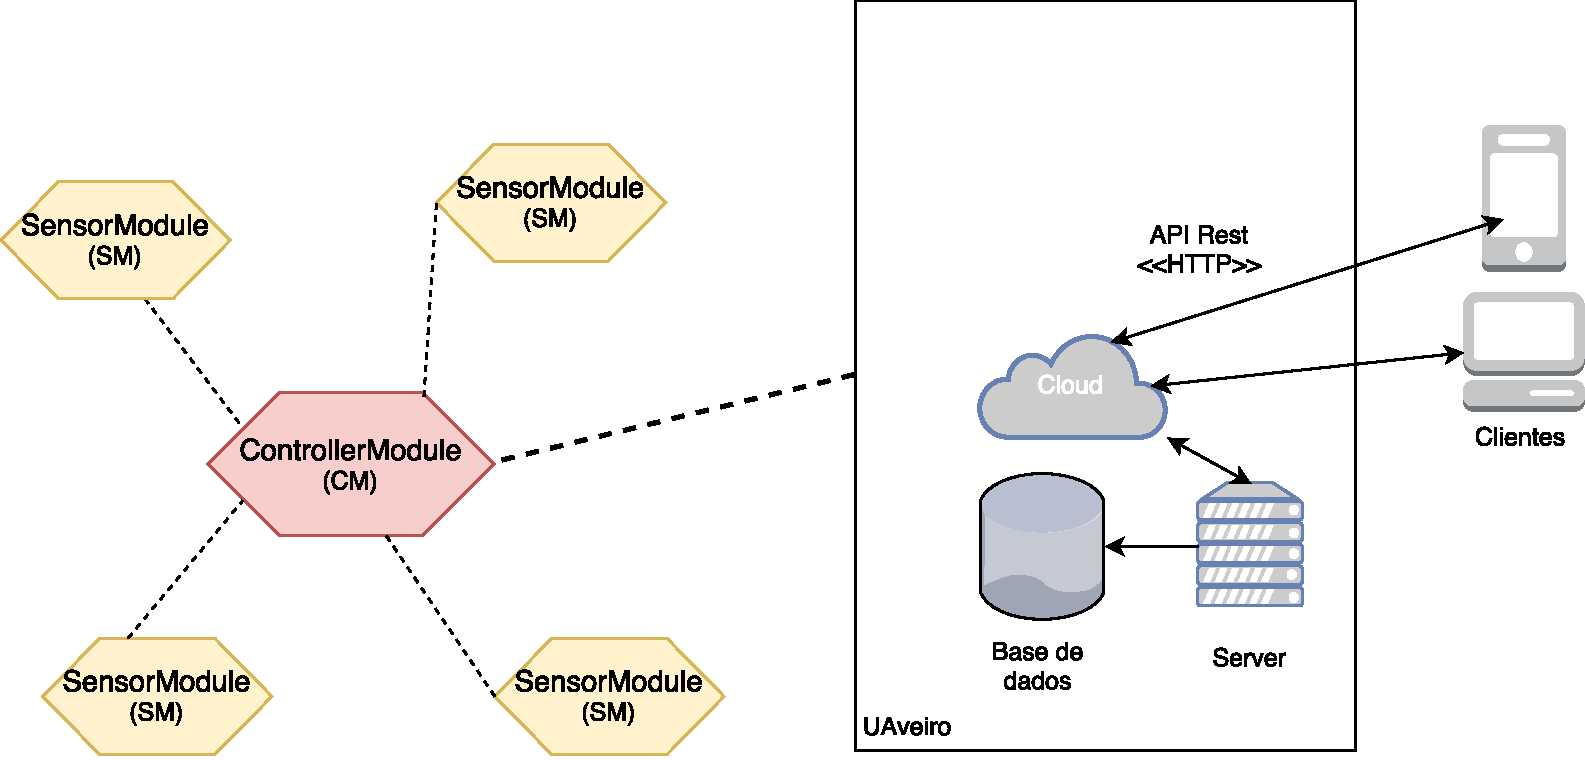
\includegraphics[scale=0.55]{esquemas/arquitetura_geral.pdf}
	\caption{Pirâmide do conhecimento: modelo DIKW}
	\label{dikw}
\end{figure}


\newpage


\section{Componentes}


\begin{figure}[!htb]
	\centering
	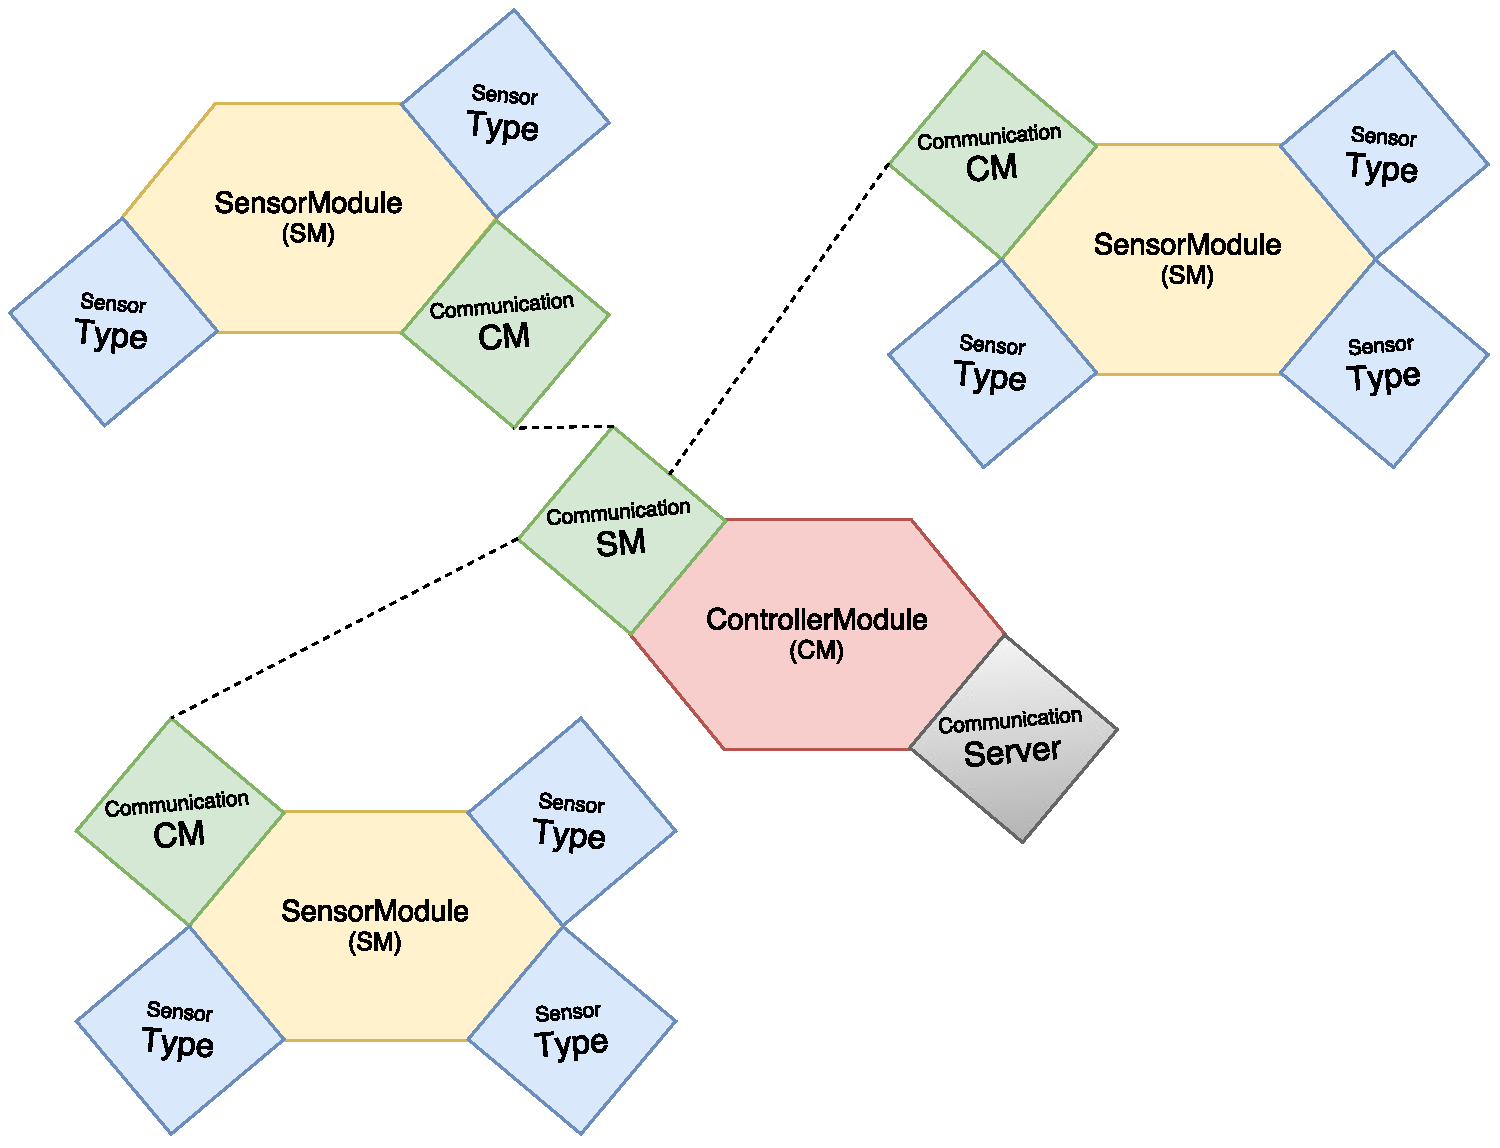
\includegraphics[scale=0.45]{esquemas/general-electronic-modules.pdf}
	\caption{Pirâmide do conhecimento: modelo DIKW}
	\label{dikw}
\end{figure}






\section{Considerações finais}